\documentclass[a4paper,12pt]{article}
\usepackage[utf8x]{inputenc}
\usepackage[T1]{fontenc}

%\usepackage[T2A]{fontenc} % jei yra kirilica
\usepackage[hmargin={30mm,15mm},vmargin={20mm,20mm},bindingoffset=0mm]{geometry}
\usepackage[onehalfspacing]{setspace}
\usepackage[colorlinks=true, linkcolor=blue, citecolor=blue, urlcolor=blue, unicode]{hyperref}

%\parindent=7mm
\renewcommand{\refname}{Literatūros sąrašas} % article
%\renewcommand{\bibname}{Literatūros sąrašas} % report
\renewcommand{\contentsname}{Turinys}
\usepackage[T1]{fontenc} 

% Lukas paketai
\usepackage{booktabs}% http://ctan.org/pkg/booktabs
\newcommand{\tabitem}{~~\llap{\textbullet}~~}
\usepackage{graphicx}
\usepackage{indentfirst}
\usepackage{setspace}
\usepackage{placeins}
\usepackage{booktabs}% http://ctan.org/pkg/booktabs
\usepackage{tabularx}% http://ctan.org/pkg/tabularx
\usepackage[parfill]{parskip}
\usepackage[unicode]{hyperref}
\usepackage{hyperref}
\usepackage{tocloft}
\usepackage{graphicx}
\newcommand\AtPageUpperRight[1]{\AtPageUpperLeft{%
   \makebox[\paperwidth][r]{#1}}}
\usepackage[dotinlabels]{titletoc}
\usepackage[capposition=top]{floatrow}
\hypersetup{
    colorlinks,
    citecolor=black,
    filecolor=black,
    linkcolor=black,
    urlcolor=black
}
\usepackage{secdot}




\begin{document}
\graphicspath{ {/} }

\renewcommand{\cftdot}{.}	
\renewcommand{\cftsecleader}{\cftdotfill{\cftdotsep}}

\thispagestyle{empty} % nerasomas psl. nr


\begin{center}
 VILNIAUS UNIVERSITETAS 
 
MATEMATIKOS IR INFORMATIKOS FAKULTETAS

MATEMATINĖS INFORMATIKOS KATEDRA

\vspace{4cm}

Projekto vadovas \ \ \textbf{Lukas Tutkus} \\
\textbf{Julius Daukšas} \\
\textbf{Dominykas Smaliukas} \\
\textbf{Robert Stankevič} \\

\vspace{0.2cm}

Bioinformatikos studijų programos grupė BioSawmill



\vspace{3cm}
\textbf{\Large Dvimatė pjovimo optimizacija}\\
\textbf{\Large Projekto planas}

\vfill

Vilnius \ \  2015
\end{center}



\clearpage

\tableofcontents
\clearpage
\section{Funkciniai ir nefunkciniai reikalavimai}
\begin{frame}
\centering

\label{my-label}
\begin{tabular}{|l|l|l|}
\hline
\textbf{ID}	& \textbf{Reikalavimai}						& \textbf{Moduliai}  \\ \hline

F1	& Registracija										& 1	     		\\ \hline

F2	& Prisijungimas prie sistemos						& 1, 3			\\ \hline

F3	& Atsijungimo nuo sistemos							& 1, 3			\\ \hline

F4	& Slaptažodžio atgavimas								& 1, 3			\\ \hline

F5	& Paskyros parametrų keitimas 	  					& 1, 3			\\ \hline 

F6	& Vartotojo paskyros deaktyvacija					& 1				\\ \hline

F7	& Vartotojo paskyros aktyvacija						& 1				\\ \hline

F8	& Vartotojo paskyros ištrinimas						& 3				\\ \hline

F9	& Pjovimo optimizacijos duomenų įvedimas				& 1, 3			\\ \hline

F10	& Pjūvio plano optimizavimas           	   			& 2				\\ \hline

F11	& Optimizuotų pjūvio planų informacijos pateikimas	& 2     			\\ \hline

F12	& Optimizuotų pjūvio planų variantų pasirinkimas		& 1, 3			\\ \hline

F13 & Pjūvio plano ruošinio atsisiuntimas				& 1, 3			\\ \hline

F14 	& Pjūvio plano informacijos išsaugojimas				& 1, 3			\\ \hline

F15	& Kalbos pasirinkimas(LT, EN)						& 1, 3			\\ \hline

NF1 & Užtikrinti kalbos pakeitimą						& 1, 3			\\ \hline

NF2 & Prisijungimo vardo ilgis nemažesnis už 4			& 1, 3			\\ \hline 

NF3 & Elektroninis paštas galioja						& 1, 3			\\ \hline 

NF3 & Slaptažodžio ilgis nemažesnis už 8					& 1, 3			\\ \hline 

NF4 & Prisijungimo duomenys išskyrus slaptažodį - unikalūs	& 1, 3			\\ \hline 

NF5 & 
\begin{tabular}[c]{@{}l@{}}
Prisijungime pakeičiamai dalyvauja sistemoje registruotas vartotojo slapyvardis\\
arba el.paštas, bei slaptažodis.			
\end{tabular}											& 1, 3			\\ \hline 


\end{tabular}
\end{frame}

\vspace{1cm}
\textbf{Moduliai} \\
1 - Vartotojų, 2 - P.O., 3 - Administratoriaus.


\vspace{1cm}
*Informacija - panelių kiekis, bendras jų plotas, likutis, pjovimo ilgis, detalių išdėstymas.

\section{Atsekamumo lentelė}
\begin{frame}
\centering
\hspace{-2cm}
\label{my-label}
\begin{tabular}{|l|c|}
\hline
\textbf{Užsakovo poreikiai}						& \textbf{Reikalavimai} 		\\ \hline

\begin{tabular}[c]{@{}l@{}}
Vartotojas nurodo reikalingų detalių ilgius (mm), 
aukščius (mm) ir kiekius.                                                                                                                                                                                                                                                                              
\end{tabular} 									& F9		                		\\ \hline

\begin{tabular}[c]{@{}l@{}}
Sistema optimizuoja detalių išpjovimą iš standartinių panelių 1200x2500.\\ 
Po to pakartoja šį procesą su standartiniais paneliais 1200x3050.\\ 
(Turėkite omenyje, kad pjovimo plotis yra 4 mm, todėl iš standartinės \\ 
panelės 1200x2500 negalima išpjauti 2 detalių 600x2500.)
\end{tabular}									& F10, F11					\\ \hline

\begin{tabular}[c]{@{}l@{}}
Sistema pateikia abiejų variantų informaciją vartotojui ir pasirenka, \\ 
kuris variantas jam labiau tinka. Vartotojui pasirinkus, sistema \\ 
turi parodyti ekrane pjovimo planą su galimybe jį atsispausdinti \\
(su atspausdintu planu vartotojas gali kreiptis į tiekėją, kad \\ 
išpjautų jam reikiamas detales).
\end{tabular}									& F12, F13	 				\\ \hline

Planuojama sistemą pateikti kaip paslaugą išoriniams vartotojams.                                                                                                                                                                                                                                                                                         												& F1, F2	, F3, F4, F5, F6	, F7	\\ \hline

Įvedami standartinių panelių dydžiai.			& F9							\\ \hline

\end{tabular}
\end{frame}

\clearpage

\section{Klasių diagramos}
\begin{frame}

\centering
\hspace{-2cm}
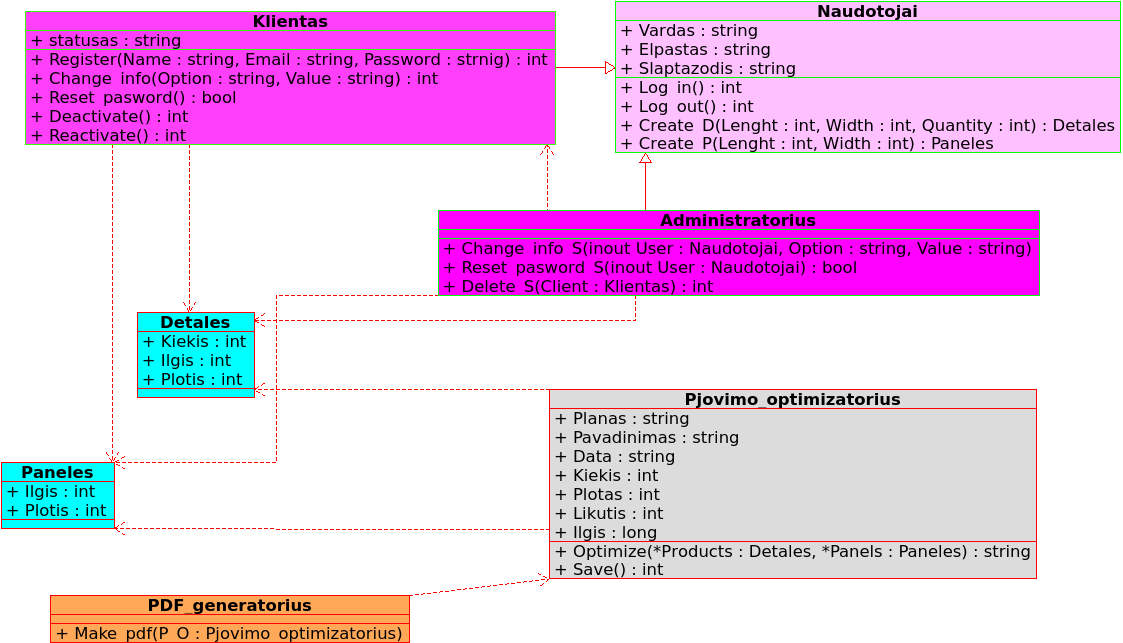
\includegraphics[width=19cm, height=19cm]{class_diagram.png}
\end{frame}

\clearpage

\section{Naudojimo atvejų aprašai(Use-cases)}
\begin{frame}
\centering
\hspace{-1cm}
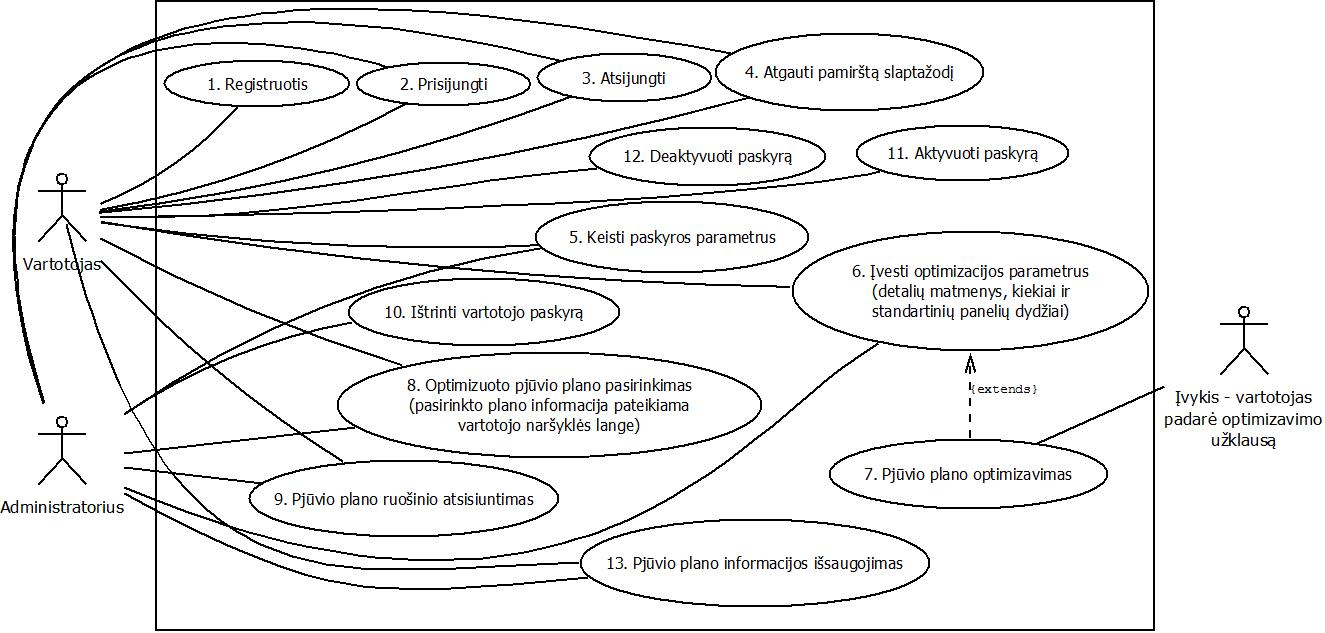
\includegraphics[width=18cm, height=14cm]{diagrama}

\end{frame}


% <<<<<<<<< USE CASES TABLE / NAUDOJIMO ATVEJU LENTELES >>>>>>>>>>>
\begin{frame}
\centering
\hspace{-1cm}
\label{my-label}
\begin{tabular}{|l|l|}
\hline
\textbf{Pavadinimas}  		& Registracija							\\ \hline
\textbf{Dalyviai}  			& Vartotojas								\\ \hline
\textbf{Paskirtis}  			& Sukurti naujo vartotojo paskyrą		\\ \hline
\textbf{Kritiškumas}			& Privalomas								\\ \hline
\textbf{Pradinės sąlygos}   	& Atidaryti tinklalapį naršyklėje		\\ \hline
\textbf{Rezultatas}   		& Sistemos duomenų bazėje sukurta 
							naujo vartotojo paskyra					\\ \hline
\textbf{
	\begin{tabular}[c]{@{}l@{}}
		Tipinė eiga ir kiti\\ 
		galimi variantai
	\end{tabular}
} &   
\begin{tabular}[c]{@{}l@{}}
	1. Vartotojas, atidaręs P.O. tinklalapį, prieš naudojantis\\
	optimizacija, turi prisiregistruoti.\\
	Registravimosi formoje privaloma užpildyti laukus: \\
	\tabitem unikalų vartotojo vardą (>=4 simboliai)\\
	\tabitem unikalų, galiojantį el.paštą (>=4 simboliai).\\
	\tabitem slaptažodį(>=8 simboliai)\\\\
	
	2. Suvedus duomenis paspausti mygtuką "Registruotis".\\\\
	
	3. Jeigu suvestas vartotojo vardas, bei paštas unikalūs duomenų bazėje,\\
	tada sukuriamas vartotojo įrašas duomenų bazėje ir vartotojas\\
	nukreipiamas į naujos paskyros langą. \\
	Jei suvestas paštas ar vartotojo vardas pasikartojo duomenų bazėje,\\
    arba neatitinka standartinio formato, vartotojui pranešama apie tai,\\
    ir laukiama, kad įvestų iš naujo.
\end{tabular} \\ \hline

\end{tabular}
\end{frame}

% <<<<<<<<<<<<<<<<<<<<<<<<<<<<<

\vspace{2cm}

\begin{frame}
\centering
\hspace{-1cm}
\label{my-label}
\begin{tabular}{|l|l|}
\hline
\textbf{Pavadinimas}  		&	Prisijungimas prie sistemos						\\ \hline
\textbf{Dalyviai}  			&	Vartotojas, administratorius						\\ \hline
\textbf{Paskirtis}  			&	Prieiga prie vartotojo paskyros, P.O. 			\\ \hline
\textbf{Kritiškumas} 		&	Privalomas										\\ \hline
\textbf{Pradinės sąlygos}	&	Naudotojo įrašas sistemos duomenų bazėje			\\ \hline
\textbf{Rezultatas}			&  	Prieiga prie savo paskyros bei P.O. atlikimas	\\ \hline
\textbf{
	\begin{tabular}[c]{@{}l@{}}
		Tipinė eiga ir kiti\\ galimi variantai
	\end{tabular}} 				&   
\begin{tabular}[c]{@{}l@{}}
1. Prisijungimo lange suvedami prisijungimo duomenis:\\ 
vartotojo vardas arba paštas ir slaptažodis.\\\\

2. Paspaudžiamas mygtukas "Prisijungti".\\\\

3. Sistema patikrina ar prisijungimo duomenys atitinka naudotojo įrašo\\
duomenis (vardą ar paštą ir slaptažodį) duomenų bazėje.\\
Naudotojas nukreipiamas į savo paskyrą jei įvesti duomenys atitiko.\\
Kitu atveju pranešama, jog prisijungimo duomenys klaidingi.\\\\

4. Atsiranda mygtukas "Istorija", sąrašas išsaugotų P.O. planų pavadinimų\\
Paspaudus pavadinimą atsiranda išsaugota informacija.\\
\end{tabular} \\ \hline

\end{tabular}
\end{frame}

% <<<<<<<<<<<<<<<<<<<<<<<<<<<<<
\vspace{1cm}
\begin{frame}
\centering
\hspace{-1cm}
\label{my-label}
\begin{tabular}{|l|l|}
\hline
\textbf{Pavadinimas}			&	Atsijungimas nuo sistemos 					\\ \hline
\textbf{Dalyviai}			&   Vartotojas, administratorius    				\\ \hline
\textbf{Paskirtis}			&  	Nutraukti sistemos naudojimosi sesiją       	\\ \hline
\textbf{Kritiškumas}			&  	Privalomas									\\ \hline
\textbf{Pradinės sąlygos}	& 	Sistemos naudotojas yra prisijungęs 
								prie sistemos   								\\ \hline
\textbf{Rezultatas}			&	Nutraukta sistemos naudotojo sesija      
\\ \hline
\textbf{
\begin{tabular}[c]{@{}l@{}}
	Tipinė eiga ir kiti\\ 
	galimi variantai
\end{tabular}} &
\begin{tabular}[c]{@{}l@{}}
	1. Paspaudžiamas mygtukas "Atsijungti", \\
	sesija baigiama.
\end{tabular} \\ \hline
\end{tabular}
\end{frame}

% <<<<<<<<<<<<<<<<<<<<<<<<<<<<<

\vspace{1cm}
\begin{frame}
\centering
\hspace{-1cm}
\label{my-label}
\begin{tabular}{|l|l|}
\hline
\textbf{Pavadinimas}			&  	Slaptažodžio atgavimas					\\ \hline
\textbf{Dalyviai}			&	Vartotojas, administratorius				\\ \hline
\textbf{Paskirtis}			&   Sužinoti pamirštą slaptažodį.			\\ \hline
\textbf{Kritiškumas}			&	Privalomas								\\ \hline
\textbf{Pradinės sąlygos}	&  								 			\\ \hline
\textbf{Rezultatas}			&	\begin{tabular}[c]{@{}l@{}}
								Naudotojas į el. paštą gauna savo \\
								slaptažodžio priminimą
								\end{tabular}   						\\ \hline
\textbf{
	\begin{tabular}[c]{@{}l@{}}
		Tipinė eiga ir kiti\\ 
		galimi variantai
	\end{tabular}
} &   
\begin{tabular}[c]{@{}l@{}}

	1. Paspaudžiamas pamiršto slaptažodžio atgavimo mygtukas "Pamiršau slaptažodį".\\\\
	
	2. Atsidariusioje formoje nurodomas el. paštas\\ 
	ar vardas, kurie yra užregistruoti sistemoje.\\\\
	 
	3. Paspaudžiamas mygtukas "Išsiūsti į paštą" ir vykdoma forma. \\\\
	
	4. Jei el. paštas ar vardas egzistuoja sistemos duomenų bazėje, tada \\ 
	išsiunčiamas laiškas su slaptažodžiu paskyros įraše esantį paštą. \\

	Jei nei vardo, nei el. pašto atitikmens nerandama duomenų bazėje,\\
	perspėjama, kad įvesti duomenys neatpažinti, pasiūloma prisiregistruoti.\\
\end{tabular} \\ \hline

\end{tabular}
\end{frame}


\begin{frame}
\centering
\hspace{-1cm}
\label{my-label}
\begin{tabular}{|l|l|}
\hline
\textbf{Pavadinimas}			&  	Paskyros parametrų keitimas						\\ \hline
\textbf{Dalyviai}			&	Vartotojas, administratorius						\\ \hline
\textbf{Paskirtis}			&	Leisti pakeisti paskyros duomenis				\\ \hline
\textbf{Kritiškumas}			& 	Neprivalomas										\\ \hline
\textbf{Pradinės sąlygos}	&  	Įvykdytas prisijungimas							\\ \hline
\textbf{Rezultatas}			&   Pakeista paskyros informacija					\\ \hline
\textbf{
	\begin{tabular}[c]{@{}l@{}}
		Tipinė eiga ir kiti\\
		galimi variantai
	\end{tabular}
} &   
\begin{tabular}[c]{@{}l@{}} 
	1. Spaudžiamas mygtukas "Redaguoti paskyrą".\\\\
	
	2. Vartotojas gali pakeisti norimus paskyros duomenis.\\
	Administratorius gali pakeisti bet kurios paskyros \\
	prisijungimo vardą, prisijungimo paštą ir tik savo \\
	paskyros slaptažodį.\\\\
	
	3. Spaudžiamas mygtukas "Išsaugoti pakeitimus".\\\\
	
	4. Pakeitimai turi atitikti registracijos formos reikalavimus: \\
	\tabitem prisijungimo vardas >= 4 simboliai\\
	\tabitem el. paštas galiojantis\\
    \tabitem slaptažodis >= 8 simboliai. \\
	Atitikus reikalavimus, pakeitimai atnaujinami paskyroje, duomenų bazėje, \\
	vardas ir el. paštas atnaujinami administratoriaus matomų paskyrų sąraše.
	Neatitikus pažymimi neleistinas reikšmes įgiję laukai.\\

\end{tabular}																	 \\ \hline

\end{tabular}
\end{frame}

\vspace{1cm}
\begin{frame}
\centering
\hspace{-1cm}
\label{my-label}
\begin{tabular}{|l|l|}
\hline
\textbf{Pavadinimas}			&  	Vartotojo paskyros deaktivacija.					\\ \hline
\textbf{Dalyviai}			&	Vartotojas										\\ \hline
\textbf{Paskirtis}			&	Deaktyvuoti nenaudojamą paskyrą					\\ \hline
\textbf{Kritiškumas}			& 	Neprivalomas										\\ \hline
\textbf{Pradinės sąlygos}	& 	Įvykdytas prisijungimas							\\ \hline
\textbf{Rezultatas}			&	Deaktyvuota vartotojo paskyra					\\ \hline
\textbf{
	\begin{tabular}[c]{@{}l@{}}
		Tipinė eiga ir kiti\\ 
		galimi variantai
	\end{tabular}
} &   
\begin{tabular}[c]{@{}l@{}} 	
	1.	Spaudžiamas mygtukas "Deaktyvuoti paskyrą".\\\\
	
	2. 	Paskyros būsena pakeičiama į "deaktyvuotą". \\
	Deaktivacijos mygtuką pakeičiamas aktyvacijos mygtuku.\\
	Deaktyvuota paskyra negali naudotis P.O.
	

\end{tabular} \\ \hline

\end{tabular}
\end{frame}


\vspace{1cm}
\begin{frame}
\centering
\hspace{-1cm}
\label{my-label}
\begin{tabular}{|l|l|}
\hline
\textbf{Pavadinimas}			&  	Vartotojo paskyros aktyvacija					\\ \hline
\textbf{Dalyviai}			&	Vartotojas										\\ \hline
\textbf{Paskirtis}			&	Aktyvuoti reikalingą paskyrą						\\ \hline
\textbf{Kritiškumas}			& 	Neprivalomas										\\ \hline
\textbf{Pradinės sąlygos}	&	Atliktas prisijungimas prie sistemos				\\ \hline
\textbf{Rezultatas}			&   Aktyvuota vartotojo paskyra 						\\ \hline
\textbf{
	\begin{tabular}[c]{@{}l@{}}
		Tipinė eiga ir kiti\\ 
		galimi variantai
	\end{tabular}
} &   
\begin{tabular}[c]{@{}l@{}} 
	1.	Spaudžiamas mygtukas "Aktyvuoti paskyrą".\\\\
	
	3. 	Paskyros būsena pakeičiama į "aktyvuotą".\\
	Aktivacijos mygtukas pakeičiamas į deaktyvacijos mygtuką.\\
	Aktyvuota paskyra vėl gali naudotis P.O.

\end{tabular} \\ \hline

\end{tabular}
\end{frame}

\begin{frame}
\centering
\hspace{-1cm}
\label{my-label}
\begin{tabular}{|l|l|}
\hline
\textbf{Pavadinimas}			&  	Vartotojo paskyros trynimas.						\\ \hline
\textbf{Dalyviai}			&	Administratorius									\\ \hline
\textbf{Paskirtis}			&	Ištrinti nenaudojamas ar kenkėjiškas paskyras	\\ \hline
\textbf{Kritiškumas}			& 	Neprivalomas										\\ \hline
\textbf{Pradinės sąlygos}	& 	Įvykdytas prisijungimas							\\ \hline
\textbf{Rezultatas}			&   Ištrintas tam tikras vartotojo įrašas        	\\ \hline
\textbf{
	\begin{tabular}[c]{@{}l@{}}
		Tipinė eiga ir kiti\\ 
		galimi variantai
	\end{tabular}
} &   
\begin{tabular}[c]{@{}l@{}} 
	1.	Pateikiamas paskyrų sarašas su visų vartotojų paskyromis(be \\
	administratoriaus paskyros).Sąraše laikomi vartotojų vardai bei el. paštai.\\ 
	Paspaudus ant tam tikros paskyros iškyla tos paskyros trinimo mygtukas.\\\\
	
	2. 	Spaudžiamas mygtukas "Trinti paskyrą".\\\\
	
	3.	Į ištrintą paskyra nusiunčiamas pranešimas, kad paskyra ištrinta.\\
	Paskyrą ištrinama iš duomenų bazės bei iš paskyrų sarašo.\\
	
	

\end{tabular} \\ \hline

\end{tabular}
\end{frame}

\vspace{1cm}

\begin{frame}
\centering
\hspace{-1cm}
\label{my-label}
\begin{tabular}{|l|l|}
\hline
\textbf{Pavadinimas}			&  	Pjovimo optimizacijos duomenų įvedimas.						\\ \hline
\textbf{Dalyviai}			&  	Vartotojas, administratorius  									\\ \hline
\textbf{Paskirtis}			&  	\begin{tabular}[c]{@{}l@{}}
									Parametrų perdavimas, pagal kuriuos algoritmas optimizuos detalių išdėstymą\\
									ant standartinių panelių
								\end{tabular}												\\ \hline
\textbf{Kritiškumas}			& 	Privalomas													\\ \hline
\textbf{Pradinės sąlygos}	& 	Aktyvuotas ir prisijungęs prie sistemos vartotojas			\\ \hline
\textbf{Rezultatas}			& 	Įvesti reikalingi parametrai optimizacijos vykdymui. \\ \hline
\textbf{
	\begin{tabular}[c]{@{}l@{}}
		Tipinė eiga ir kiti\\ 
		galimi variantai
	\end{tabular}
} &   
\begin{tabular}[c]{@{}l@{}} 
	1. Optimizacijos formoje pateikiami pasirenkami/atšaukiami\\
	standartiniai panelių dydžiai (1200x2500, 1200x3050), o žemiau \\
	jų galima įvesti papildomų panelių matmenis. Optimizacija vyks\\
	tik tada kai bus pasirinkta ar įvesta bent vienos panelės išmatavimai.\\\\
	
	2. Taip pat nurodomi reikalingų detalių:\\
		ilgiai (mm),	 aukščiai (mm) ir kiekiai.\\
	Taip pat galima įkelti '.xlsx' formato failą, su ilgio, aukščio ir \\
	kiekio stulpeliais.\\\\
	
	3. Detalių duomenys nurodomi sveikaisiais skaičiais, jų kiekis \\
	ne didesnis nei 1000. Ilgiai, aukščiai mažesni ar lygūs\\
	nurodytų standartinių panelių matminims. Standartinės \\
	panelės matmenys galimi nuo 10mm iki 20000mm, o maksimalus \\
	kiekis - 10. \\\\
	
	4. Paspaudžiamas "Optimizuoti" mygtukas ir optimizacija vyksta jei visi \\
	duomenys teisingi pagal 3 dalies reikalavimus. \\
	Kitu atveju vartotojui pranešama, kuris reikalavimas neišpildytas.\\
\end{tabular} \\ \hline

\end{tabular}
\end{frame}

\vspace{1cm}

\begin{frame}
\centering
\hspace{-1cm}
\label{my-label}
\begin{tabular}{|l|l|}
\hline
\textbf{Pavadinimas}				&	Pjūvio plano optimizavimas		\\ \hline
\textbf{Dalyviai}				&	Vartotojas, administratorius		\\ \hline
\textbf{Paskirtis}				&	Optimizuoti pjovimo planą 		\\ \hline
\textbf{Kritiškumas}				& 	Privalomas						\\ \hline
\textbf{Pradinės sąlygos}		& 	Atliktas pjovimo optimizacijos 
									duomenų įvedimas 				\\ \hline
\textbf{Rezultatas}				&  	Surandamas optimizuotas pjovimo 
									planas/planai.  					\\ \hline
\textbf{
	\begin{tabular}[c]{@{}l@{}}
		Tipinė eiga ir kiti\\ 
		galimi variantai
	\end{tabular}
} &   
\begin{tabular}[c]{@{}l@{}} 
	1. Optimizuojamas pjovimo planas/planai, stengiantis panaudoti kuo mažiau panelių.\\
	Planų kiekis priklauso nuo įvestų skirtingų standartinių\\
	panelių dydžių.\\\\

	3. Pateikiamas optimizacijos rezultatas.
\end{tabular} \\ \hline

\end{tabular}
\end{frame}

% <<<<<<<<<<<<<<<<<<<<<<<<<<<<<

\vspace{1cm}
\begin{frame}
\centering
\hspace{-1cm}
\label{my-label}
\begin{tabular}{|l|l|}
\hline
\textbf{Pavadinimas}					&	Optimizuoto pjūvio plano pasirinkimas						\\ \hline
\textbf{Dalyviai}					&	Vartotojas, administratorius    								\\ \hline
\textbf{Paskirtis}					&  	Pasirinktas P.O. planas galės būti išsaugotas ar atsisiųstas.\\ \hline
\textbf{Kritiškumas}					& 	Privalomas													\\ \hline
\textbf{Pradinės sąlygos}			& 
\begin{tabular}[c]{@{}l@{}}
	Sistema baigusi optimizuoti pjūvio planus/planą pagal \\
	nurodytus optimizacijos parametrus. \\
\end{tabular} 																						\\ \hline
\textbf{Rezultatas}					&   \begin{tabular}[c]{@{}l@{}} 
												Pasirinktą pjūvio planą galima atsisiųsti ar \\
												išsisaugoti
										\end{tabular}     \\ \hline
\textbf{
\begin{tabular}[c]{@{}l@{}}
	Tipinė eiga ir kiti\\ galimi variantai
\end{tabular}} 						&   
\begin{tabular}[c]{@{}l@{}} 
	1. Pasirenkamas vienas iš pateiktų pjovimo planų.\\
	pagal pateiktą informaciją: panelių kiekį, bendras jų plotą,\\
	likutį, detalių išdėstymą, bendrą pjovimo ilgį.\\\\


	2. Pasirinkus pjovimo planą atsiranda mygtukai: \\
	"Atsisiųsti" - atsisiųsti optimizacijos plano ruošinį, \\
	"Išsaugoti" - išsaugoti optimizacijos plano informaciją. \\
	
\end{tabular} \\ \hline
\end{tabular}
\end{frame}

% <<<<<<<<<<<<<<<<<<<<<<<<<<<<<
\vspace{1cm}
\begin{frame}
\centering
\hspace{-1cm}
\label{my-label}
\begin{tabular}{|l|l|}
\hline
\textbf{Pavadinimas}			& 	Pasirinkto pjūvio plano ruošinio atsisiuntimas	\\ \hline
\textbf{Dalyviai}			&   Vartotojas, administratorius						\\ \hline
\textbf{Paskirtis}			&  	Pateikti atsisiuntimui paruoštą pjūvio planą.	\\ \hline
\textbf{Kritiškumas}			& 	Privalomas										\\ \hline
\textbf{Pradinės sąlygos}	& 	Pasirinktas Optimizuoto pjūvio planas.			\\ \hline
\textbf{Rezultatas}			&   Atsisiunčiamas pjūvio planas. 					\\ \hline
\textbf{	
	\begin{tabular}[c]{@{}l@{}}
		Tipinė eiga ir kiti\\ 
		galimi variantai
	\end{tabular}
} &	
\begin{tabular}[c]{@{}l@{}} 
	1. Spaudžiamas mygtukas "Atsisiųsti"\\\\
	
	2. Į naudotojo prietaisą nusiunčiamas pjūvio planas \\
	".pdf" formatu, kurį jis galės spausdintis.
\end{tabular} \\ \hline

\end{tabular}
\end{frame}

\vspace{1cm}

\begin{frame}
\centering
\hspace{-1cm}
\label{my-label}
\begin{tabular}{|l|l|}
\hline
\textbf{Pavadinimas}			& 	Pjūvio plano informacijos išsaugojimas.			\\ \hline
\textbf{Dalyviai}			&   Vartotojas, administratorius						\\ \hline
\textbf{Paskirtis}			&  	Išsaugoti pasirinktą pjūvio planą				\\ \hline
\textbf{Kritiškumas}			& 	Privalomas										\\ \hline
\textbf{Pradinės sąlygos}	& 	Pasirinktas Optimizuoto pjūvio planas.			\\ \hline
\textbf{Rezultatas}			&   Išsaugotas pasirinktas pjūvio planas			 	\\ \hline
\textbf{
	\begin{tabular}[c]{@{}l@{}}
		Tipinė eiga ir kiti\\ 
		galimi variantai
	\end{tabular}
} &	
\begin{tabular}[c]{@{}l@{}} 
	1 	Įvedamas pjūvio plano pavadinimas.\\\\
	
	2.	Paspaudžiamas mygtukas "Išsaugoti" .\\\\
	
	3. 	Į duomenų bazę išsaugoma pjūvio plano informacija:\\
	įvestas pavadinimas, data, panelių kiekis, bendras jų plotas,\\
	likuts, detalių išdėstymas,	bendras pjovimo ilgis.\\\\

	4. 	Pjovimo optimizacijos "Istorija" sąraše atsiranda nauja P.O.\\
	Paspaudus pjūvio plano pavadinimą parodoma išsaugotą informaciją.\\
	
\end{tabular} \\ \hline

\end{tabular}
\end{frame}

\clearpage

\section{Sistemos elgsenos aprašymas}
\vspace{1cm}

\begin{frame}
\centering
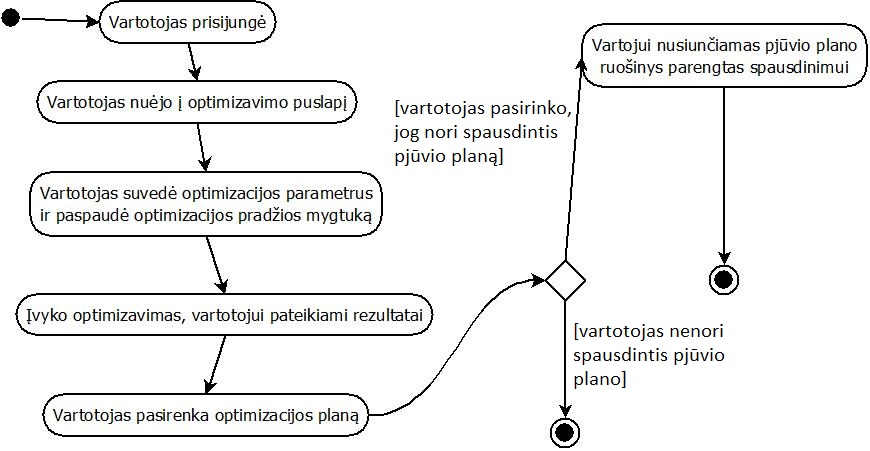
\includegraphics[width=18cm, height=10cm]{swim}

\end{frame}


\begin{frame}
\centering
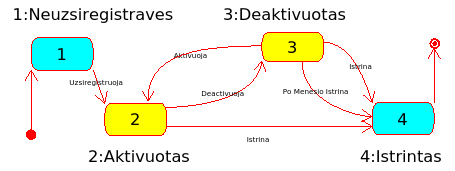
\includegraphics[width=15cm, height=10cm]{state_diagram.png}

\end{frame}

\end{document}
